\documentclass{lkx_pset}

\title{Math 213b Problem Set 1}
\author{Lev Kruglyak}
\due{January 31, 2024}

\usepackage{graphicx}

\newcommand{\D}{\mathbb{D}}
\newcommand{\x}{\mathbf{x}}
\usepackage{pgfplots}
\pgfplotsset{
	compat=1.12,
}


\collaborator{AJ LaMotta}
\collaborator{Jarell Cheong}

\begin{document}
\maketitle
\collaborators

\begin{problem}{1}
  Recall from class that an end $e$ of a topogical space $X$ is an assignment of a path component $e(K)$ of the complement $X\setminus K$ for every compact subset $K\subset X$ subject to the requirement that inclusions are preserved in reverse: i.e. if $K'\subset K$, then $e(K')\subset e(K)$.
\end{problem}

\begin{parts}
  \begin{part}{a}
    Using the definition, show fairly carefully that the real line $\R$ has two ends while $\R^2$ has only one end.
  \end{part}

  Let's begin by showing that $\R$ has at least $2$ ends. Assume that $K\subset \R$ is a compact subset. By the Heine-Borel theorem, the points $\inf(K)$ and $\sup(K)$ must both exist, and be in $K$. Now we can construct two distinct ends. Let's define $e_1(K) = (-\infty, \inf(K))$ and $e_2(K) = (\sup(K), \infty)$ and $e_1(\emptyset) = e_2(\emptyset)=\R$. These clearly satisfy the conditions to be an end.

  To show that there are at most two ends, note that any end $e$ of $\R$ must send $e(\emptyset) = \R$. Then $e(\{p\})$ is either $(-\infty, p)$ or $(p, \infty)$ since $\R\setminus \{p\}$. The first case corresponds to $e_1$ and the second corresponds to $e_2$. In both cases, expanding $[p-\epsilon, p+\epsilon]$ gives full equality with one of $e_1$ or $e_2$.

  In the case of $\R^2$, we can note that $\R^2\setminus \{p\}$ is connected, so a similar argument shows that all ends are equal to the end $e$ which sends $\{p\}$ to the path connected component $\R^2\setminus \{p\}$, and extending naturally from there.

  \begin{part}{b}
    Suggest what you think the classification should be for connected, orientable
    2-manifolds with three ends. No proof required. Feel free to look up the classification of surfaces with finitely many ends.
  \end{part}

  Intuitively, given some connected, orientable 2-manifold with three ends, we can compactify each of the ends to get a connected orientable $2$-manifold. In the case that this resulting manifold is compact, such manifolds are entirely classified by their genus, i.e. they are homeomorphic to $X_g$ for some genus $g$. This means that the connected, orientable 2-manifolds are exactly the trice-punctured genus $g$ surfaces $X_g - \{p_1, p_2, p_3\}$ for three distinct points $p_i$. We might propose an extension of this classification which also allows for infinite genera.
\end{parts}

\begin{problem}{2}
  The following figure depicts part of a doubly-periodic surface $X$, extending in-
  finitely across the plane.
\end{problem}

\begin{solution}
  \begin{center}
    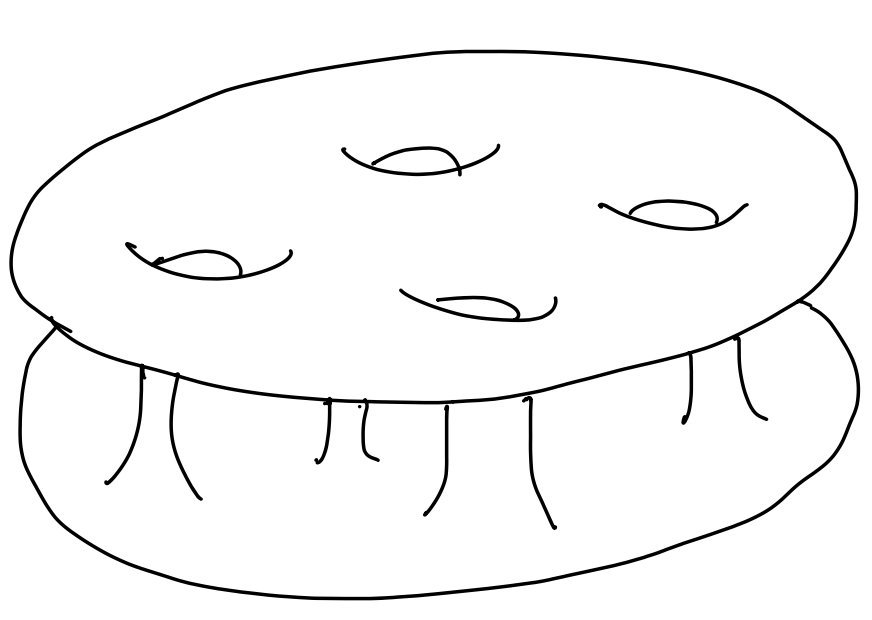
\includegraphics[scale=0.5]{figure1.png}
  \end{center}
  \begin{part}{a}
    Exhibit a subset of $X$ that is homeomorphic to a genus-1 surface with one boundary component (i.e. a closed genus-1 surface with a disk removed).
  \end{part}

  We can cut out the following surface from $X$:
  \begin{center}
    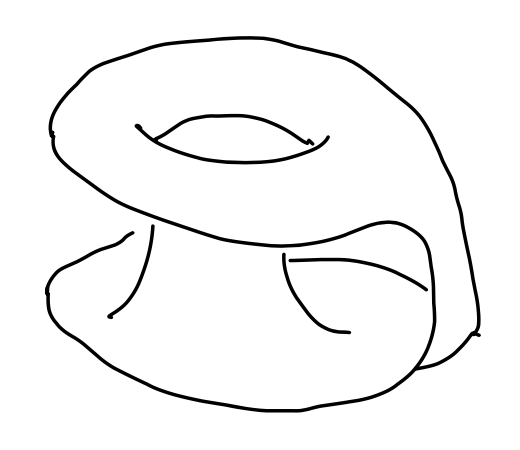
\includegraphics[scale=0.5]{figure2.png}
  \end{center}

  \begin{part}{b}
    Exhibit a subset of $X$ that is diffeomorphic to a genus-4 surface with one boundary component (i.e. a closed genus-4 surface with a disk removed).
  \end{part}

  Similarly we can cut out the following surface from $X$:
  \begin{center}
    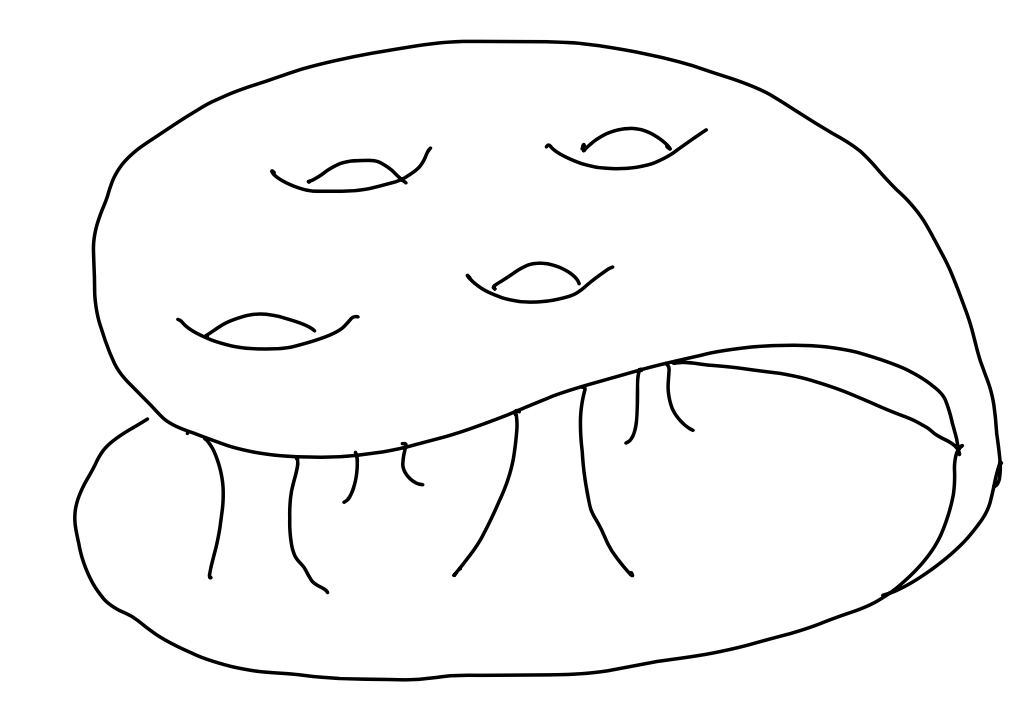
\includegraphics[scale=0.5]{figure3.png}
  \end{center}
\end{solution}

\begin{problem}{3}
  Algebraic curves.
\end{problem}

\begin{parts}
  \begin{part}{a}
  Let $X \subset \mathbb{C}^2$ be the affine algebraic curve defined by $z^n + w^n = 1$. Show that $X$ is indeed a smooth curve. Let $\phi : X \rightarrow \mathbb{C}$ be the projection to the $z$ axis. Find the branch points and ramification points (aka critical points and critical values) of $ \phi $ and the order of the branch points.
  \end{part}

  Note that $X$ is the zero locus of the polynomial $P =z^n+w^n-1\in \C[z, w]$. This has derivative $(\partial P/\partial z, \partial P/\partial w)=(nz^{n-1}, nw^{n-1})$ at a point $(z,w)$. Since this is nonzero at every point of $X$, $X$ is a smooth curve.

  To find the critical points of the projection of $\phi$, we are looking for points $(z,w)\in X$ with $\partial P/\partial w = 0$. This means solving
  \[
    \begin{cases}
      z^n + w^n=1,\\ nw^{n-1}=0,
    \end{cases} \quad\implies \quad (z,w) = (e^{2\pi i k/n})\quad\textrm{for}\quad k\in \{1, \ldots, n\}.
  \]
  In local coordinates $w$ around these critical points, the projection function has the form $(1-w^n)^{1/n}\approx z' + (z'/n)w^n + O(w^{n+1})$. Thus, the critical points have order $n$, and the critical values are
  \[
  \varphi(e^{2\pi i k / n}, 0) = e^{2\pi i k /n}.
  \]

  \begin{part}{b}
  Let $ Y \subset \mathbb{C}^2 $ be the curve $ w^2 = z^3 - z $. Let $ \psi : Y \rightarrow \mathbb{C} $ be the projection to the $ w $ axis. Find the branch points and ramification points of $ \psi $ and the order of the branch points.
  \end{part}
  In this case, the curve is the zero locus of the polynomial $Q = w^2-(z^3-z)\in \C[z, w]$. Now the derivative is $(\partial Q/\partial z, \partial Q/\partial w)=(-3z^2+1, 2w)$. The only zeroes of this derivative are $(\sqrt{1/3}, 0), (-\sqrt{1/3}, 0)$, which are not on the curve so $Y$ is a smooth curve.

  We do the same thing as in the previous part to get the critical points 
  \[
    \left(-\frac{\sqrt{3}}{3}, \pm\frac{\sqrt{2}}{3^{3/4}}\right), 
    \left(\frac{\sqrt{3}}{3}, \pm\frac{i\sqrt{2}}{3^{3/4}}\right).
  \]
  It's slightly tedious to show that these points have all order $2$, and we can check that the critical values are $\pm \sqrt{2}/3^{3/4}$, $\pm i\sqrt{2}/3^{3/4}$.
\end{parts}

\begin{problem}{4}
Show that any non-constant holomorphic map $ f : \mathbb{CP}^1 \rightarrow \mathbb{CP}^1 $ arises as a rational function: a ratio of polynomials $ f(z) = p(z)/q(z) $, in the standard coordinate $ z $ on $ \mathbb{C} \subset \mathbb{CP}^1 $. You might do this by induction on the degree of $ f $, interpreted as the number of zeros counted with multiplicity.
\end{problem}

\begin{solution}
  Suppose $f : \CP^1 \to \CP^1$ is a non-constant holomorphic map, equivalently $f$ can be interpreted as a meromorphic function $f: \CP^1 \to \C$. Since it is non-constant, the poles of $f$ have to be isolated; otherwise in a neighborhood around a pole which is an accumulation pole, the classical identity theorem would imply that the function is identically zero. Next, compcatness of $\CP^1$ implies that there are only a finite amount of zeroes, since any infinite sequence in a compact space must have a convergent subsequence, with limit a pole as well. This contradicts the isolation of the poles.

  Now let's assume without loss of generality that $\infty$ is not a pole of $f$, say the poles are $p_1,\ldots, p_n\in \C$. Now consider the function
  \[
    g(z) = f(z) - \sum_{1\leq i\leq n} \mathcal{PP}_{f}(p_i, z) \quad\textrm{where}\quad \mathcal{PP}_{f}(p_i, z)=\sum_{1\leq j\leq \mathrm{ord}(p_i)} \alpha_{-j}\cdot \frac{1}{(z-p_i)^j}
  \]
  is the series of principal parts of $f$ at $p_i$. Then by construction $g$ is a holomorphic map $\CP^1 \to \C$. Since $\CP^1$ is compact, any such function $g$ achieves its maximum, and by the maxmimum principle this implies that $g$ is constant. Thus, $f$ is equal to the sum of principal parts series and is thus a rational function.
\end{solution}

\begin{problem}{5}
Let $ S \subset \mathbb{C}^2 $ be the zero set of a smooth function $ F : \mathbb{C}^2 \rightarrow \mathbb{C} $ and assume that $ F(z, w) $ is a holomorphic function of both $ z $ and $ w $. Do not assume anything else about $ F $; in particular, we do not assume that $ S $ is smooth. Show that $ S $ has no isolated points. That is, every point of $ S $ is a limit point.
\end{problem}

\begin{solution}
  Let's assume for the sake of contradiction that $F$ has an isolated zero $(z_0, w_0)\in S$, and let's say $B_\epsilon$ is some polydisk of radius $\epsilon>0$ centered at $(z_0, w_0)$, with $F$ nonzero on $\overline{B_\epsilon}\setminus \{(z_0, w_0)\}$. Now for every $w\in \C$ with $|w-w_0|<\epsilon$, let's define
  \[
    f(w) = \frac{1}{2\pi i}\oint_{|z-z_0|=\epsilon} \frac{\partial F(z, w)/ \partial z}{F(z, w)}\,dz.
  \]
  By the argument principle, $f(w)$ counts the number of zeroes of $F(z,w) : \C \to \C$ with $|z-z_0|<\epsilon$. Since $f$ is continuous, and we know by construction that $f(w)=0$ for all $w\neq w_0$, it follows by continuity that $f(w_0)=0$ as well. This is a contradiction.
\end{solution}

\end{document}
